\documentclass[11pt,a4paper]{article}
\usepackage[margin=2.4cm]{geometry}
\usepackage{amsmath,amssymb,bm}
\usepackage{booktabs}
\usepackage{siunitx}
\usepackage{enumitem}
\usepackage{graphicx}
\graphicspath{{matlab/figs/}}
\usepackage[hidelinks]{hyperref}

\sisetup{detect-all}
\newcommand{\T}{^{\top}}

\title{Ride-Height Control of a Fully Submerged Hydrofoil Boat:\\
LQR with Integral Action and a Kalman Filter}
\author{ELEC3304 Control --- Assessment 2\\[2pt]
Group members: \emph{(name 1)}, \emph{(name 2)}}
\date{October 2026}

\begin{document}
\maketitle

\noindent This document continues \emph{model\_derivation.pdf}, which derives the
nonlinear model, the trim point and the LTI model
$\dot{\bm x}=A\bm x+B\tilde{\bm u}+E\bm w$, $\bm y=C\bm x$ with
$\bm x=[\,h\;\;v\;\;\theta\;\;q\,]\T$, two foil inputs and three measurements
(bow height, pitch angle, pitch rate). Section~\ref{sec:log} records the design
decisions that changed during the work and the trade-offs behind them.

\section{Objectives and specifications}

The controller must hold the boat at a commanded ride height with the hull
level, using only the three sensors, in the presence of waves and of errors in
the model. We translate this into the following specifications, checked on the
nonlinear model with actuator limits:

\begin{enumerate}[label=S\arabic*.,leftmargin=2.4em]
\item \textbf{Stability}: the open-loop plant has an unstable pole; all
      closed-loop poles must lie in the left half-plane, also for speeds
      6--\SI{9}{m/s} and masses 190--\SI{240}{kg}.
\item \textbf{Tracking}: a \SI{5}{cm} height step settles (2\,\%) within about
      \SI{2}{s} with less than \SI{10}{\percent} overshoot.
\item \textbf{Zero steady-state error} in height and pitch when the speed or the
      mass differs from the design values.
\item \textbf{Actuator limits}: in normal operation the foil deflection stays
      inside the \SI{+3.5}{\degree} upward margin available at trim, and the rate
      inside \SI{20}{\degree/s}.
\item \textbf{Disturbance rejection}: in regular head waves (\SI{5}{cm}
      amplitude) the height error stays well below the \SI{15}{cm} range in which
      the linear model is valid.
\end{enumerate}

\section{Controller}
\label{sec:control}

\subsection{Structure}

The controller is an LQR state feedback with integral action on two outputs, a
reference feedforward and a reference prefilter. All quantities are deviations
from trim:
\begin{align}
\tilde{\bm u} &= \bm N_u r_f - K\bigl(\hat{\bm x} - \bm N_x r_f\bigr) - K_i\,\bm\xi,
\label{eq:law}\\
\dot{\bm\xi} &= \begin{bmatrix}\hat h - r_f\\ y_2\end{bmatrix},
\qquad
\dot r_f = \frac{r - r_f}{t_f}.
\label{eq:int}
\end{align}
Here $r$ is the commanded height change, $r_f$ its filtered version,
$\hat{\bm x}$ the estimate from the observer of Section~\ref{sec:obs}, and
$y_2$ the measured pitch angle. The terms have the following roles:
\begin{itemize}
\item $K(\hat{\bm x}-\bm N_x r_f)$ stabilises the boat and drives the state to
      its target.
\item $K_i\bm\xi$ removes steady-state errors in height and pitch caused by model
      errors (specification S3). Two integrators are needed because there are two
      outputs to hold; Section~\ref{sec:log} explains why the height integrator
      acts on the estimate $\hat h$ and not on the raw ultrasonic reading.
\item $\bm N_x$, $\bm N_u$ give the steady state that corresponds to a height
      $r$ with level pitch, obtained from
      $\begin{bmatrix}A & B\\ C_z & 0\end{bmatrix}
       \begin{bmatrix}\bm N_x\\ \bm N_u\end{bmatrix}
       =\begin{bmatrix}\bm 0\\ [1\;\;0]\T\end{bmatrix}$ with
      $C_z=\begin{bmatrix}1&0&0&0\\0&0&1&0\end{bmatrix}$.
      They let the controller move directly to the new height instead of waiting
      for the integrators.
\item The prefilter with $t_f=\SI{0.3}{s}$ turns a step command into a smooth
      one, which keeps the foil deflection small (Section~\ref{sec:log}).
\item \textbf{Anti-windup}: whenever the commanded foil angle exceeds the position
      limit, $\dot{\bm\xi}$ is set to zero (integrator clamping).
\end{itemize}

\subsection{LQR design}

The gains minimise
$J=\int_0^\infty \bigl(\bm x_a\T Q\,\bm x_a + \tilde{\bm u}\T R\,\tilde{\bm u}\bigr)\,dt$
for the augmented model $\bm x_a=[\,\bm x;\bm\xi\,]$,
\[
A_a=\begin{bmatrix}A & 0\\ C_z & 0\end{bmatrix},\qquad
B_a=\begin{bmatrix}B\\ 0\end{bmatrix},
\]
which is controllable (rank 6). The weights follow Bryson's rule, each diagonal
entry being the inverse square of the largest acceptable value
(Table~\ref{tab:weights}); the two integral weights were then increased by a
factor of 10 to speed up the removal of steady-state errors.

\begin{table}[htbp]
\centering
\caption{LQR weights (Bryson's rule).}
\label{tab:weights}
\begin{tabular}{@{}llll@{}}
\toprule
Weighted quantity & Acceptable value & Weight & Note \\ \midrule
heave $h$ & \SI{2}{cm} & $1/0.02^2$ & \\
heave rate $v$ & \SI{0.5}{m/s} & $1/0.5^2$ & \\
pitch $\theta$ & \SI{2}{\degree} & $1/(2^\circ)^2$ & \\
pitch rate $q$ & \SI{10}{\degree/s} & $1/(10^\circ)^2$ & \\
$\int(h-r)$ & --- & $10/0.02^2$ & tuned \\
$\int\theta$ & --- & $10/(1^\circ)^2$ & tuned \\
each foil deflection & \SI{3}{\degree} & $1/(3^\circ)^2$ & margin is \SI{3.5}{\degree} \\
\bottomrule
\end{tabular}
\end{table}

The resulting gains (angles in rad, lengths in m) are
\[
K=\begin{bmatrix}3.284 & 0.188 & 2.788 & 0.183\\ 1.648 & 0.098 & -2.788 & -0.212\end{bmatrix},\qquad
K_i=\begin{bmatrix}7.443 & 4.155\\ 3.626 & -8.529\end{bmatrix},
\]
and the closed-loop poles of the augmented system are
$-3.32$, $-3.90\pm2.35\mathrm{j}$, $-10.83\pm5.60\mathrm{j}$ and $-18.50$.
The gain structure is physical: a height error is corrected by both foils in
the same direction (first column of $K$ positive in both rows), while a pitch
error is corrected by moving the foils in opposite directions (third column of
opposite sign).

\subsection{Results with full-state feedback}

Before adding the observer the controller was tested with the true state, to
separate the two designs.

\paragraph{Step response (Figure~\ref{fig:lqrstep}).} A \SI{5}{cm} step settles
in \SI{0.72}{s} with \SI{1.9}{\percent} overshoot on the linear model; the
nonlinear model with actuator limits is almost identical and the peak foil
deflections are \SI{1.5}{\degree} (front) and \SI{1.1}{\degree} (rear), well
inside the margin. S2 and S4 are met.

\begin{figure}[htbp]
\centering
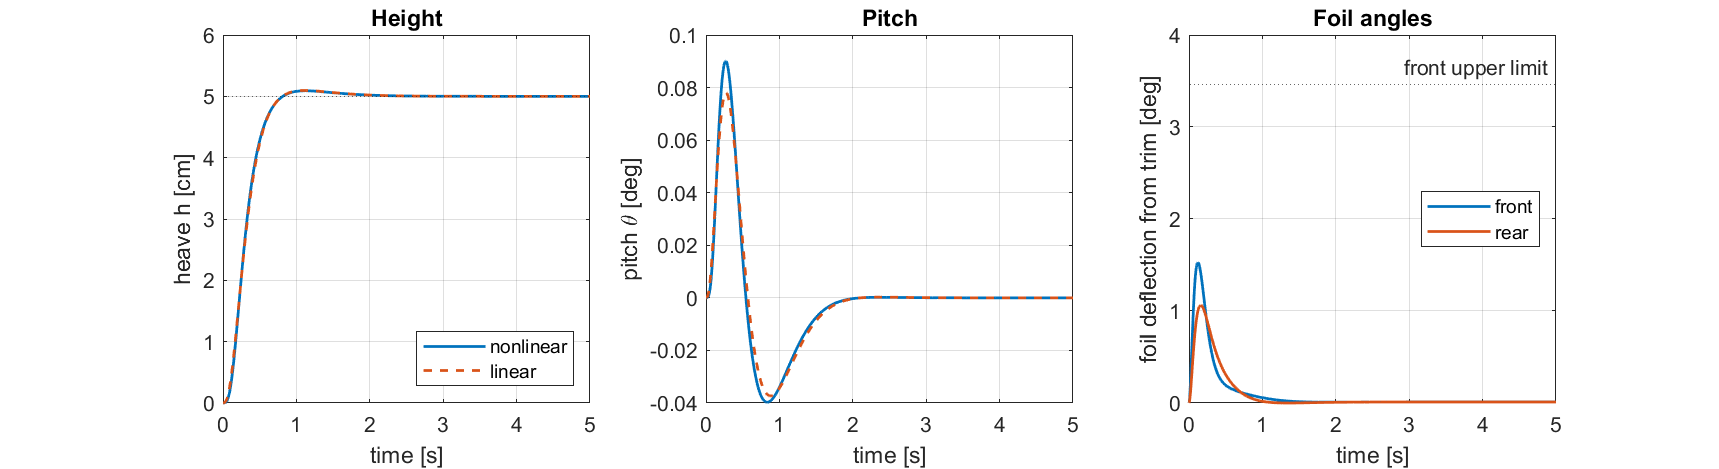
\includegraphics[width=\textwidth]{fig7_lqr_step.png}
\caption{\SI{5}{cm} height step with full-state LQR: linear and nonlinear model.}
\label{fig:lqrstep}
\end{figure}

\paragraph{Waves (Figure~\ref{fig:lqrwaves}).} In regular head waves the open-loop
boat drifts away, whereas the controlled boat holds the height within
\SI{0.18}{cm} rms and the pitch within \SI{0.20}{\degree} rms, with foil
deflections up to \SI{1.3}{\degree}.

\begin{figure}[htbp]
\centering
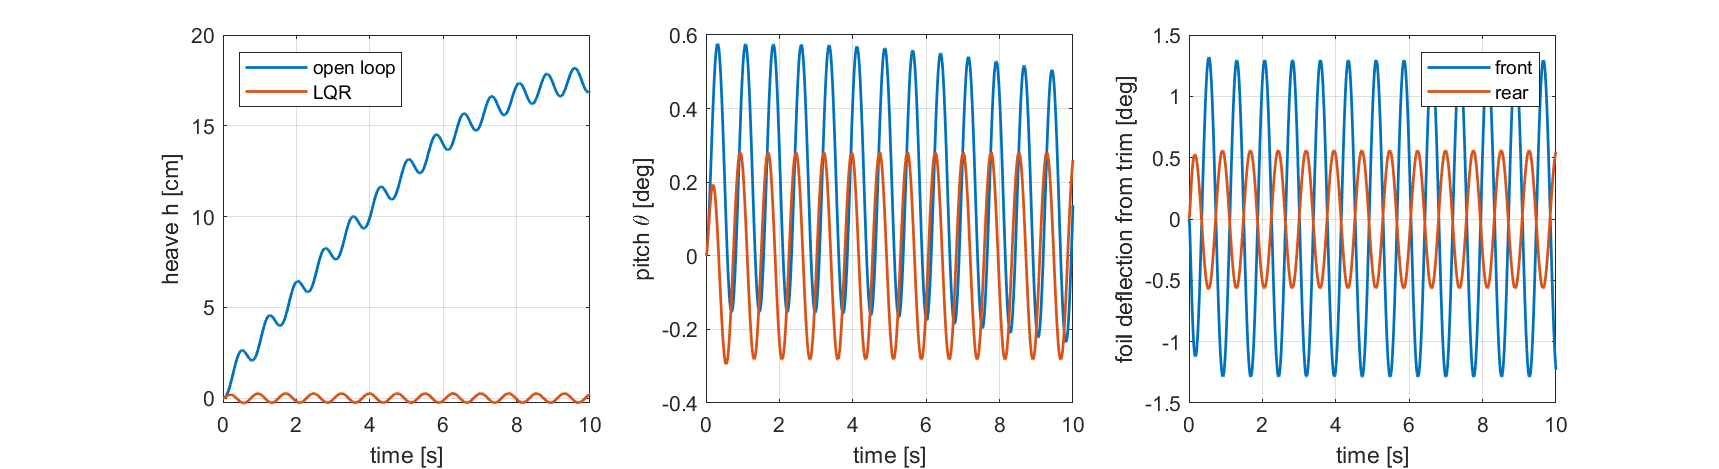
\includegraphics[width=\textwidth]{fig8_lqr_waves.png}
\caption{Regular head waves: open loop and full-state LQR.}
\label{fig:lqrwaves}
\end{figure}

\paragraph{Robustness (Figure~\ref{fig:lqrrob}).} With the nominal gains, the
closed loop of the true linearised plant is stable over the whole grid
$U=5.9$--\SI{9}{m/s}, $m=190$--\SI{240}{kg}; the slowest pole is $-3.17$.
In nonlinear simulation, a speed of 6 or \SI{8}{m/s} causes an initial
disturbance of at most \SI{1.5}{cm}, which the integrators remove within about a
second.

\begin{figure}[htbp]
\centering
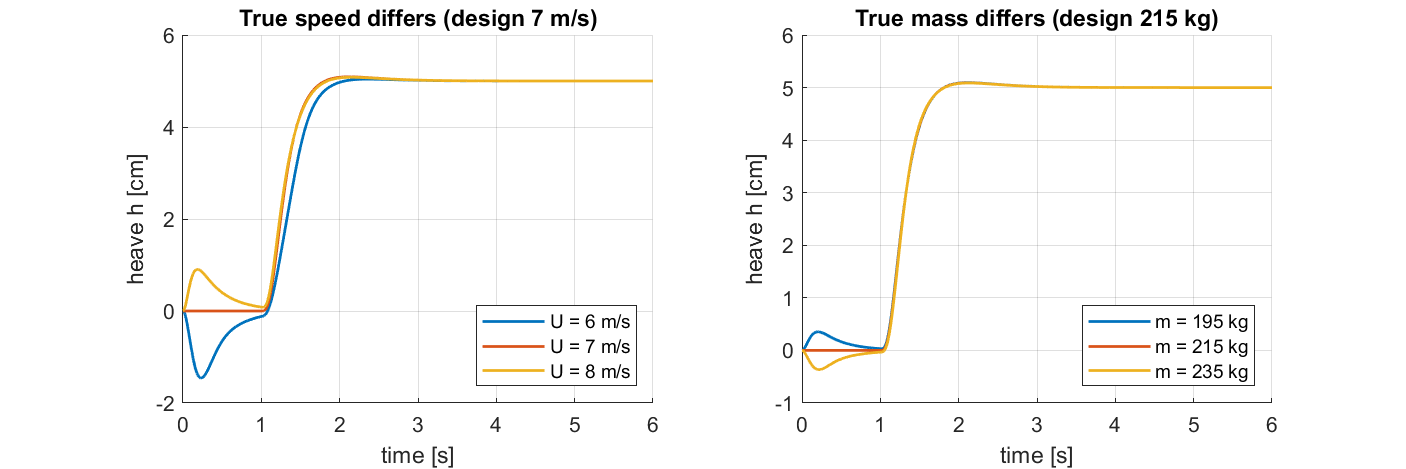
\includegraphics[width=0.85\textwidth]{fig9_lqr_robustness.png}
\caption{\SI{5}{cm} step with speed and mass different from the design values
(full-state LQR, trim inputs for the nominal values).}
\label{fig:lqrrob}
\end{figure}

\paragraph{Saturation (Figure~\ref{fig:lqrsat}).} A \SI{20}{cm} step without
prefilter drives the front foil to its \SI{7}{\degree} limit. Without
anti-windup the integrators keep growing during saturation and the height
overshoots by \SI{8.7}{cm}; with clamping the overshoot is \SI{1.0}{cm}.

\begin{figure}[htbp]
\centering
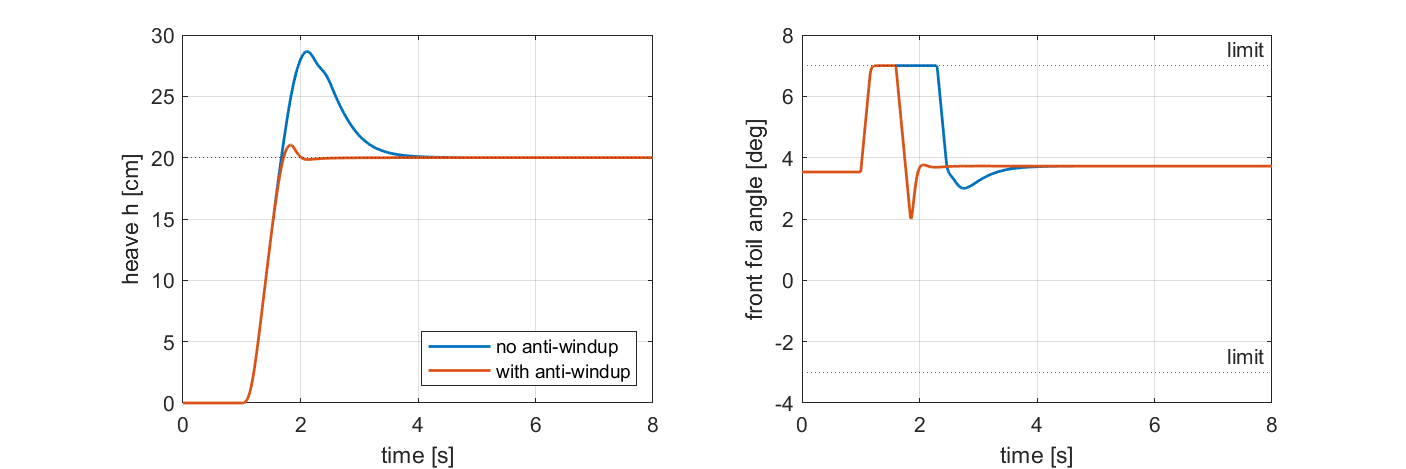
\includegraphics[width=0.85\textwidth]{fig10_lqr_saturation.png}
\caption{\SI{20}{cm} step without prefilter: effect of anti-windup.}
\label{fig:lqrsat}
\end{figure}

\section{Observer}
\label{sec:obs}

\subsection{Kalman filter with a bias state}

The observer is a steady-state Kalman filter for the model augmented with one
extra state $b$, an unknown constant vertical acceleration:
\begin{equation}
\bm x_e=\begin{bmatrix}\bm x\\ b\end{bmatrix},\qquad
\dot{\bm x}_e = A_e\bm x_e + B_e\tilde{\bm u} + L\,(\bm y - C_e\bm x_e),
\qquad
A_e=\begin{bmatrix}A & \bm e_2\\ 0 & 0\end{bmatrix},\;
B_e=\begin{bmatrix}B\\ 0\end{bmatrix},\;
C_e=\begin{bmatrix}C & 0\end{bmatrix},
\end{equation}
with $\bm e_2=[0\;1\;0\;0]\T$. The input $\tilde{\bm u}$ is the \emph{applied}
foil angle, read from the actuator encoders, so the observer stays correct when
the actuators saturate. The bias state represents what speed and mass errors do
to the boat: the front and rear lift change in the same proportion, which is a
pure vertical force with no pitching moment. The augmented pair $(A_e,C_e)$ is
observable (rank 5).

\subsection{Noise model}

\begin{itemize}
\item \textbf{Process noise}: the wave velocities $w_f,w_r$ enter through $E$,
      with variance $(0.11)^2/2$ and an assumed correlation time of \SI{0.1}{s};
      the bias follows a random walk of intensity $b_{\mathrm{rate}}^2$ with
      $b_{\mathrm{rate}}=\SI{1}{m/s^2/\sqrt{s}}$.
\item \textbf{Measurement noise}: for the AHRS and the gyro, sampled noise of
      variance $\sigma^2$ at $T_s=\SI{0.02}{s}$ gives an intensity
      $\sigma^2T_s$. The ultrasonic reading also contains the wave surface under
      the bow, of variance $\zeta_a^2/2$. Its power is concentrated in a band of
      roughly $\Delta f=\SI{0.25}{Hz}$ around the encounter frequency, so its
      spectral density there is $\zeta_a^2/(4\Delta f)$, about 100 times the value
      obtained by treating it as white noise over the sensor bandwidth. We use
      this larger value.
\end{itemize}

The resulting observer poles are $-0.67$, $-0.93\pm0.90\mathrm{j}$, $-12.0$ and
$-287$. The fast poles belong to the pitch states, which are measured directly;
the slow ones belong to the heave and the bias, which are inferred mainly from
the wave-contaminated height reading.

\subsection{Separation principle}

With the observer in the loop, the closed-loop poles of the linear system
(plant, observer and integrators, 11 states) were computed directly; they equal
the LQR poles together with the observer poles to within $6\times10^{-13}$, as
the separation principle predicts. The controller and the observer can
therefore be designed independently, and the closed loop is stable.

\subsection{Results with output feedback}

\paragraph{Estimation (Figure~\ref{fig:est}).} With waves and sensor noise, after
the initial transient the rms estimation errors are \SI{0.50}{cm} in heave,
\SI{1.0}{cm/s} in heave rate, \SI{0.045}{\degree} in pitch and
\SI{0.23}{\degree/s} in pitch rate. The heave estimate follows the true heave and
ignores the much larger oscillation of the bow-height reading, which is mostly
the water surface.

\begin{figure}[htbp]
\centering
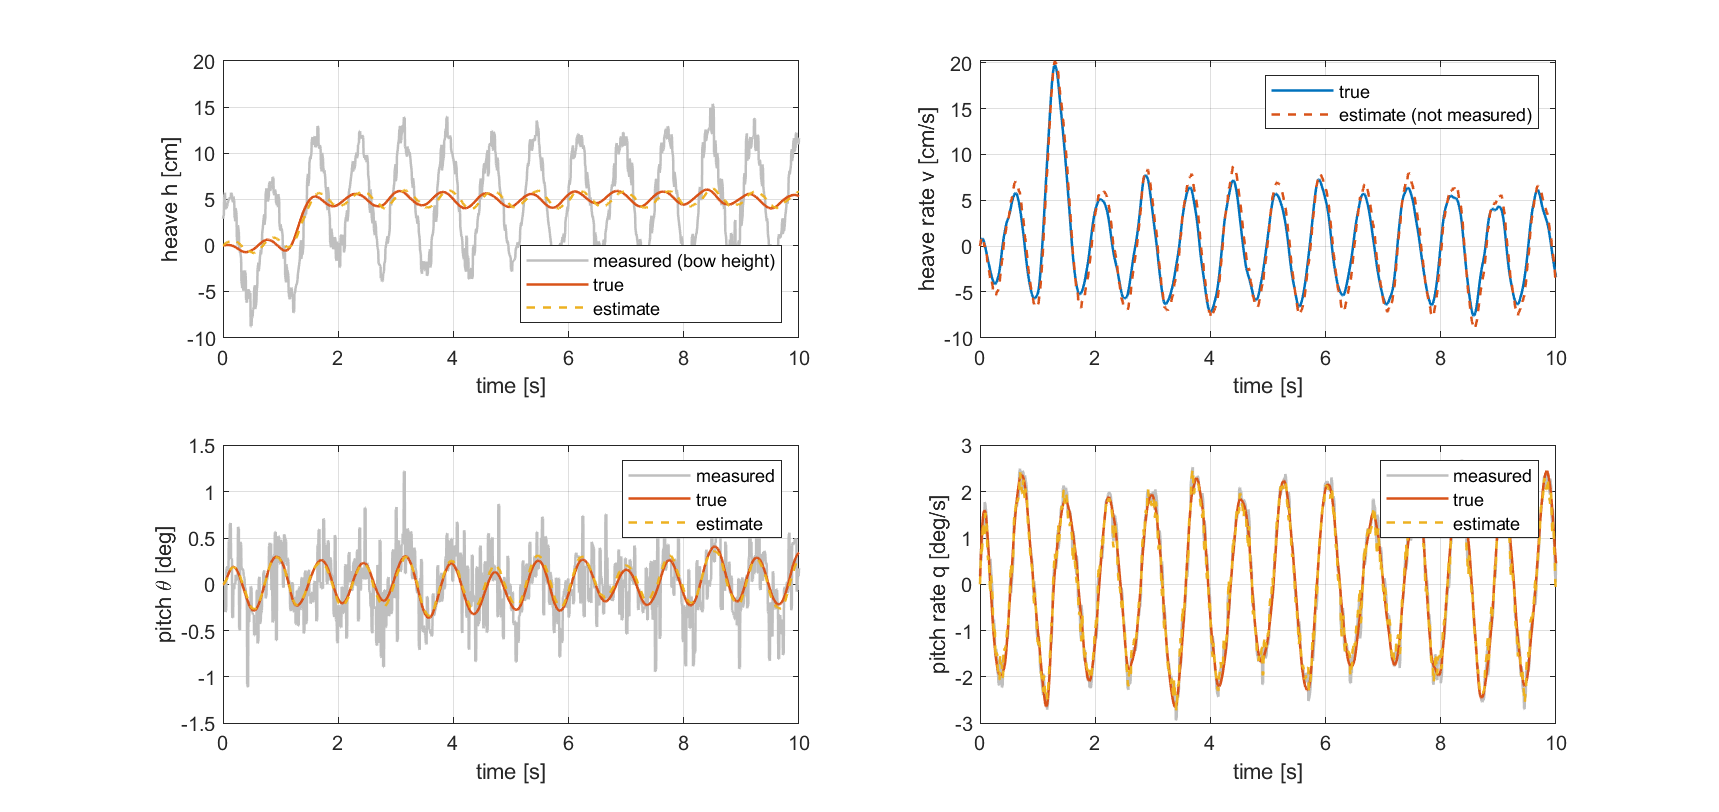
\includegraphics[width=\textwidth]{fig11_observer_estimates.png}
\caption{True, estimated and measured states during a \SI{5}{cm} step in waves
with sensor noise. The heave rate is not measured.}
\label{fig:est}
\end{figure}

\paragraph{Output vs full-state feedback (Figure~\ref{fig:ofb}).} Under the same
step, waves and noise, the height error after settling is \SI{0.56}{cm} rms with
the observer against \SI{0.18}{cm} with the true state; the pitch is the same
(\SI{0.19}{\degree} vs \SI{0.21}{\degree}). The price of estimation is a larger
foil activity: the front foil peaks at \SI{3.4}{\degree}, close to the
\SI{3.5}{\degree} margin.

\begin{figure}[htbp]
\centering
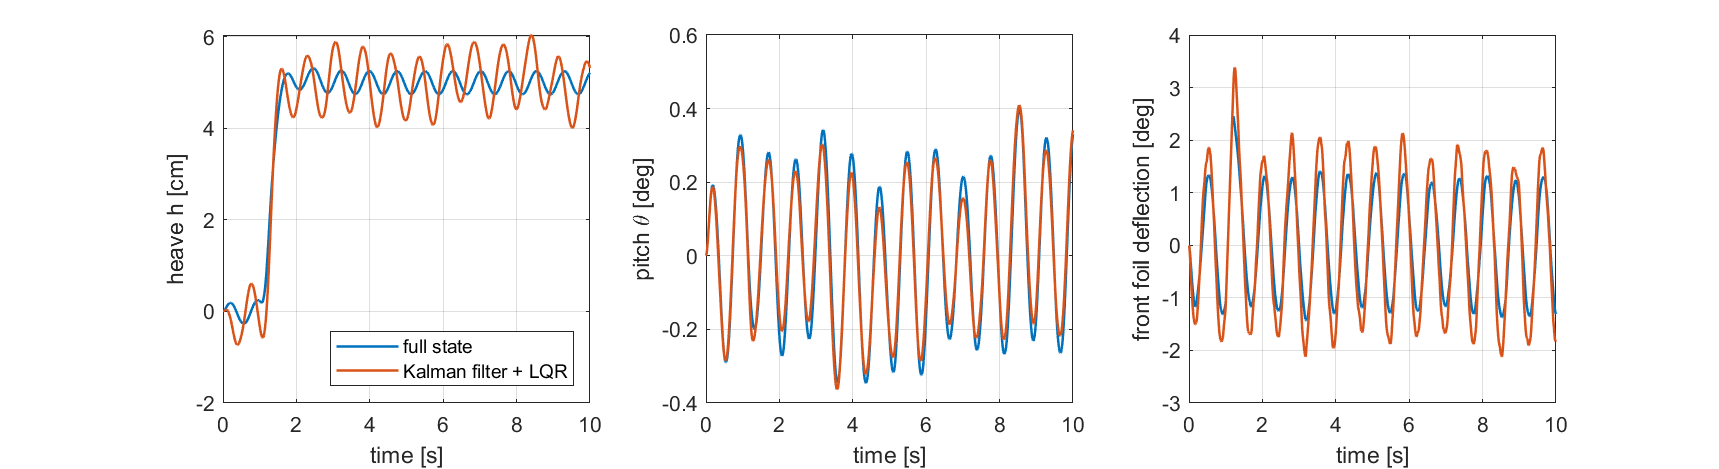
\includegraphics[width=\textwidth]{fig12_output_vs_full_state.png}
\caption{Kalman filter + LQR compared with full-state LQR, \SI{5}{cm} step in
waves with sensor noise.}
\label{fig:ofb}
\end{figure}

\paragraph{Robustness (Figure~\ref{fig:ofbrob}).} The output-feedback loop is
stable over the same speed and mass grid; its slowest pole is the slowest
observer pole, $-0.67$. In nonlinear simulation the final height and pitch are
exact for speeds of 6 and \SI{8}{m/s} and masses of 195 and \SI{235}{kg}
(specification S3). The transient is larger than with full-state feedback: a
speed \SI{1}{m/s} too low makes the boat drop by about \SI{11}{cm} before the
bias estimate catches up, after about \SI{5}{s}. The right panel shows the bias
state converging to the force caused by the speed error.

\begin{figure}[htbp]
\centering
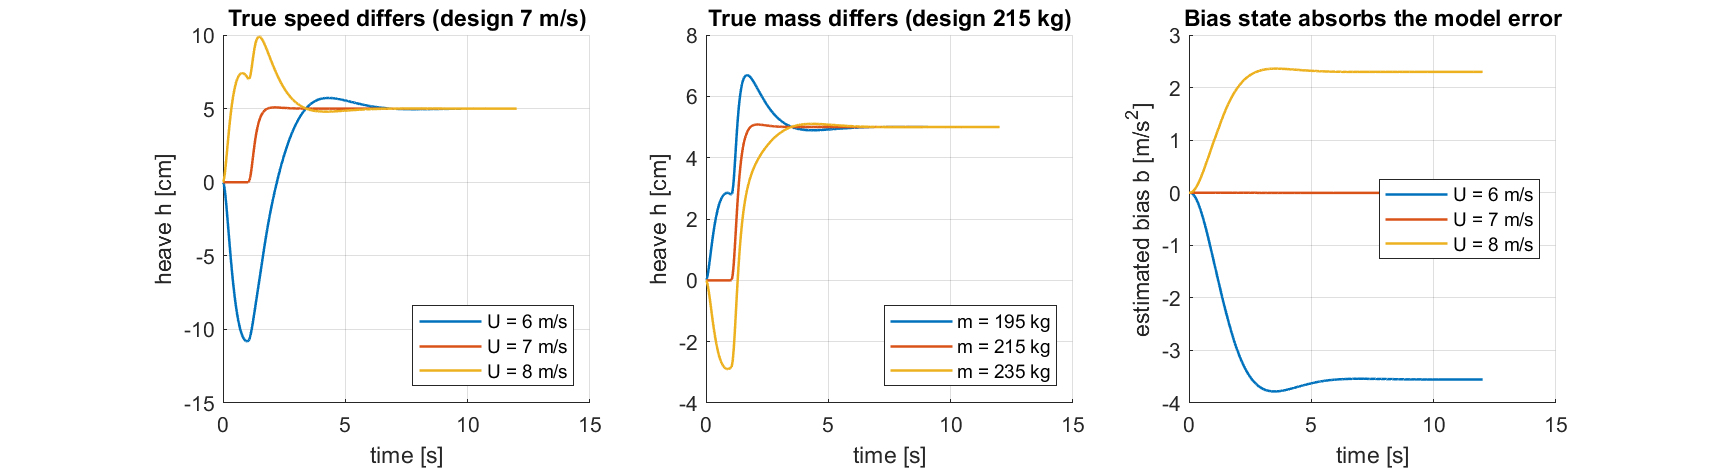
\includegraphics[width=\textwidth]{fig13_output_feedback_robustness.png}
\caption{Output feedback with speed and mass errors, and the estimated bias.}
\label{fig:ofbrob}
\end{figure}

\section{Digital implementation}
\label{sec:digital}

The real controller runs on a microcontroller: it reads the sensors at
discrete instants, computes, and sends a command that the actuators hold until
the next update. This section moves the continuous design to a sampling rate of
\SI{50}{Hz} ($T_s=\SI{20}{ms}$), the rate assumed for the sensors.

\subsection{Why the continuous design cannot simply be sampled}

The simplest route, ``emulation'', runs the continuous controller and observer
equations with a numerical integration step of $T_s$. This fails here. The
continuous Kalman filter has a pole at \SI{-287}{rad/s}, associated with the
pitch-rate gyro, which is faster than the Nyquist frequency
$\pi/T_s=\SI{157}{rad/s}$. Integrated with forward Euler at \SI{50}{Hz}, the
observer has a discrete pole of magnitude 4.74 and diverges. The observer
therefore has to be designed for the sampled system directly.

\subsection{Direct digital design}

The plant is discretised with a zero-order hold,
$\bm x_{k+1}=A_d\bm x_k+B_d\tilde{\bm u}_k$, and both designs are repeated in
discrete time with the same weights and noise intensities as before:
\begin{itemize}
\item \textbf{Discrete LQR} (\texttt{dlqr}) on $[\bm x;\bm\xi]$, with the
      integrators updated as $\bm\xi_{k+1}=\bm\xi_k+T_s[\hat h_k-r_{f,k};\,y_{2,k}]$
      and cost weights $QT_s$, $RT_s$.
\item \textbf{Discrete Kalman filter} (\texttt{dlqe}) in current-estimator form.
      The process-noise covariance is the exact discretisation of the continuous
      intensity (Van Loan's method), and the measurement covariance is the
      continuous intensity divided by $T_s$.
\end{itemize}
Each sample, the controller performs five steps:
\begin{align*}
\hat{\bm x}_{k|k-1} &= A_{de}\hat{\bm x}_{k-1|k-1}+B_{de}\bigl(\bar{\bm\delta}_{k}-\bm u_0\bigr)
  && \text{predict}\\
\hat{\bm x}_{k|k} &= \hat{\bm x}_{k|k-1}+M\bigl(\bm y_k-C_e\hat{\bm x}_{k|k-1}\bigr)
  && \text{correct}\\
\tilde{\bm u}_k &= \bm N_u r_{f,k}-K_d(\hat{\bm x}_{k|k}-\bm N_x r_{f,k})-K_{i,d}\bm\xi_k-K_u\tilde{\bm u}_{k-1}
  && \text{control law}\\
\bm\xi_{k+1} &= \bm\xi_k+T_s\bigl[\hat h_{k|k}-r_{f,k};\;y_{2,k}\bigr]
  && \text{integrate}\\
r_{f,k+1} &= a\,r_{f,k}+(1-a)\,r_k,\quad a=e^{-T_s/t_f}
  && \text{prefilter}
\end{align*}
Here $\bar{\bm\delta}_k$ is the mean of the encoder readings at the start and
end of the last interval, the integrators are frozen while the command is
saturated, and the term $K_u\tilde{\bm u}_{k-1}$ appears only in the
delay-compensated design of Section~\ref{sec:delay}. The equivalent continuous poles of the digital LQR,
$\ln z/T_s$, match the continuous design to within \SI{1}{\percent}
($-3.32$, $-3.90\pm2.35\mathrm{j}$, $-10.8\pm5.6\mathrm{j}$, $-18.4$). For the
Kalman filter the very fast pitch-rate pole moves from $-287$ to
\SI{-178}{rad/s} (a discrete pole at $z=0.03$), the complex pair and the pole at
$-12$ are unchanged, and the slowest pole moves from $-0.67$ to $-1.28$. The
digital feedback gains are 10--\SI{15}{\percent} smaller than the continuous ones.

\subsection{Computation delay}
\label{sec:delay}

A microcontroller needs time to compute, so the command calculated from the
measurements at $t_k$ is usually sent at $t_{k+1}$. We compared three cases on
the nonlinear model with sampled sensors and a zero-order-hold output: no
delay, a one-sample delay that the design ignores, and a one-sample delay
included in the design model as an extra state $\tilde{\bm u}_{k-1}$
(Table~\ref{tab:digital}).

\begin{table}[htbp]
\centering
\caption{Continuous and \SI{50}{Hz} digital controllers: \SI{5}{cm} step in
\SI{5}{cm} waves with sensor noise (errors after \SI{3}{s}), and the calm-water
step.}
\label{tab:digital}
\small
\begin{tabular}{@{}lccccc@{}}
\toprule
Controller & $h$ error & $\theta$ & front foil & \multicolumn{2}{c}{calm-water step} \\
 & (cm rms) & (deg rms) & peak (deg) & settling (s) & overshoot \\ \midrule
Continuous ($t_f=\SI{0.3}{s}$) & 0.56 & 0.19 & 3.38 & 0.72 & \SI{1.6}{\percent} \\
Digital, no delay & 0.61 & 0.21 & 2.85 & 2.17 & 0 \\
Digital, delay not compensated & 0.78 & 0.24 & 3.36 & 2.17 & 0 \\
Digital, delay compensated (chosen) & 0.74 & 0.26 & 3.34 & 2.12 & 0 \\
\bottomrule
\end{tabular}
\end{table}

With the digital prefilter of \SI{0.6}{s} (Section~\ref{sec:log}, D10), a
one-sample delay costs about \SI{0.15}{cm} of height accuracy, and compensating
for it in the design recovers only part of that. The delay matters much more
when the foils are close to saturation (D10). We keep the compensated design,
since it is the one whose design model matches the implementation.

Figure~\ref{fig:digital} shows the result. The middle panel zooms into half a
second: the command changes every \SI{20}{ms} and the servo follows it with its
lag and rate limit. The right panel shows the \SI{50}{Hz} bow-height samples,
dominated by the water surface, and the heave estimate updated at the same rate.

\begin{figure}[htbp]
\centering
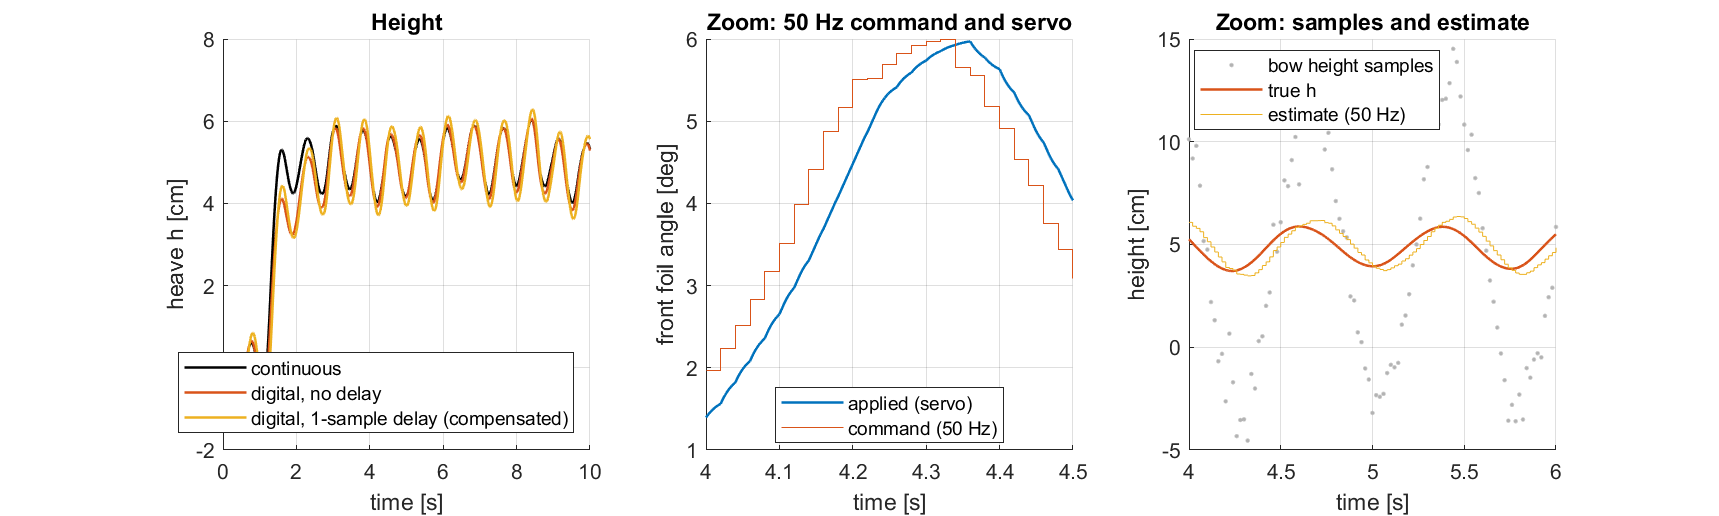
\includegraphics[width=\textwidth]{fig15_digital_vs_continuous.png}
\caption{Continuous and \SI{50}{Hz} digital controllers in waves with sensor
noise. Middle: \SI{50}{Hz} command and servo response. Right: sensor samples,
true heave and estimate.}
\label{fig:digital}
\end{figure}

\subsection{Sampling rate}

Table~\ref{tab:rate} and Figure~\ref{fig:rate} repeat the test with the
delay-compensated design re-done for each rate (sensors sampled at the same
rate, one-sample delay). The linear designs are stable down to \SI{10}{Hz}, but
on the nonlinear model with waves the front foil exceeds its upward margin at
\SI{25}{Hz} and below, and the height error quadruples. At \SI{25}{Hz} the
estimation error is the same as at \SI{50}{Hz} (\SI{0.5}{cm}), so the loss comes
from the longer hold and delay in the control loop, not from the observer. At \SI{10}{Hz} the boat drifts by
about \SI{20}{cm}. A rate of \SI{50}{Hz} is the lowest of those tested that keeps
the foils inside their range; \SI{100}{Hz} gains a further \SI{0.1}{cm}.

\begin{table}[htbp]
\centering
\caption{Effect of the controller rate (\SI{5}{cm} step in waves with noise,
one-sample delay, delay-compensated design for each rate).}
\label{tab:rate}
\begin{tabular}{@{}rcccc@{}}
\toprule
Rate (Hz) & $h$ error (cm rms) & $\theta$ (deg rms) & front foil peak (deg) & largest $|z|$ \\ \midrule
100 & 0.61 & 0.21 & 3.00 & 0.991 \\
50 & 0.74 & 0.26 & 3.34 & 0.982 \\
25 & 2.99 & 0.72 & 4.77 & 0.963 \\
20 & 2.85 & 0.72 & 5.26 & 0.955 \\
15 & 2.69 & 0.68 & 4.87 & 0.940 \\
10 & 19.7 & 0.49 & 3.46 & 0.911 \\
\bottomrule
\end{tabular}
\end{table}

\begin{figure}[htbp]
\centering
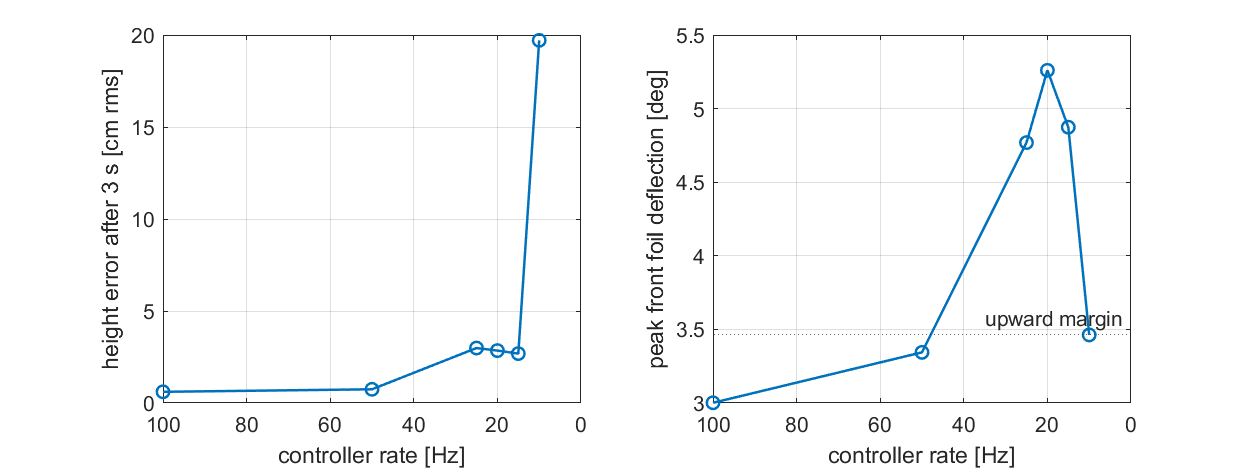
\includegraphics[width=0.85\textwidth]{fig16_sample_rate.png}
\caption{Height error and peak front-foil deflection against controller rate.}
\label{fig:rate}
\end{figure}

\subsection{Robustness of the digital loop}

The linear closed loop of the sampled plant, digital controller and one-sample
delay (13 states) was checked over the same grid of speeds and masses as
before; the largest pole magnitude is 0.984, so the loop is stable everywhere.
In nonlinear simulation, speeds of 6 and \SI{8}{m/s} and masses of 195 and
\SI{235}{kg} again give zero steady-state error in height and pitch
(Figure~\ref{fig:digrob}).

\begin{figure}[htbp]
\centering
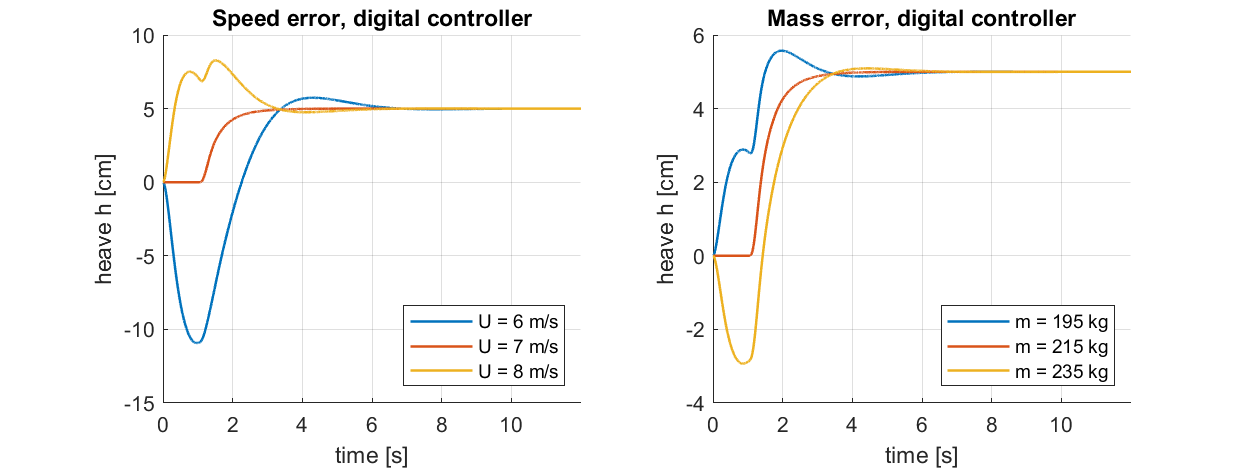
\includegraphics[width=0.85\textwidth]{fig17_digital_robustness.png}
\caption{\SI{50}{Hz} digital controller with speed and mass errors.}
\label{fig:digrob}
\end{figure}

\subsection{Simulink implementation}

In \texttt{hydrofoil\_sim.slx} the controller is an atomic subsystem with sample
time \SI{20}{ms}. Its inputs are sampled at each tick and its output is held in
between, which is the zero-order hold of the real hardware. The algorithm is in
a MATLAB Function block that calls \texttt{digital\_controller.m}: the five
steps above, written as they would be on the microcontroller. The encoder input
passes through a memory block, so the controller reads the foil angle from
before its own new command; without it, the ideal-actuator option created an
algebraic loop. In waves without noise the Simulink model and the MATLAB
simulation agree to within \SI{1.9}{mm} in heave; the difference comes from the
encoder reading being one solver step old. With noise the height error is
\SI{0.78}{cm} rms and the pitch \SI{0.24}{\degree} rms (Figure~\ref{fig:slx}).

\begin{figure}[htbp]
\centering
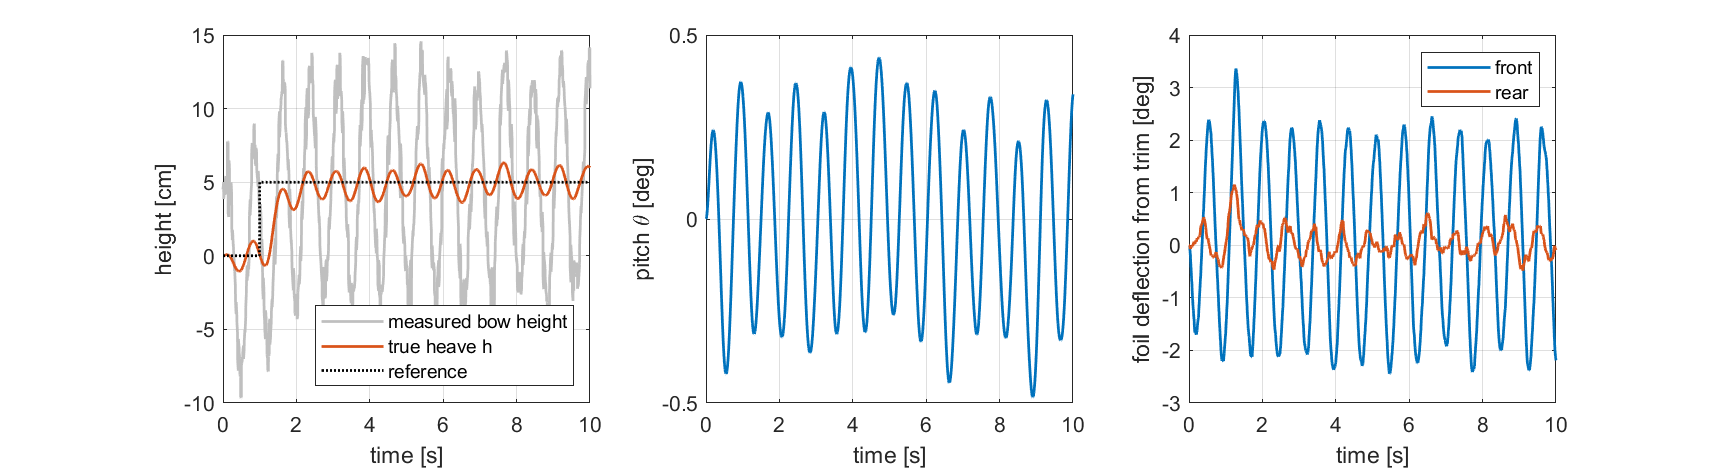
\includegraphics[width=\textwidth]{fig14_simulink_closed_loop.png}
\caption{Simulink model with the \SI{50}{Hz} digital controller: \SI{5}{cm} step
in waves with sensor noise.}
\label{fig:slx}
\end{figure}

\section{Design decisions and trade-offs}
\label{sec:log}

The final design was not the first one. Each change below was made because a
simulation showed that the earlier choice failed a specification. We record the
problem, the evidence, the alternatives considered and the cost of the chosen
option.

\subsection{D1. Reference prefilter}

\textbf{Problem.} With a step command, the feedforward and the proportional
terms act instantly. \textbf{Evidence.} Without the prefilter the \SI{5}{cm} step
has \SI{20.7}{\percent} overshoot and asks for \SI{8.9}{\degree} of front-foil
deflection, far beyond the \SI{3.5}{\degree} margin. \textbf{Decision.} A
first-order prefilter with $t_f=\SI{0.3}{s}$: overshoot \SI{1.9}{\percent}, peak
deflection \SI{1.3}{\degree}, settling time \SI{0.72}{s}. \textbf{Cost.} None
in disturbance rejection, since the prefilter acts only on the reference.
The alternative, reducing all gains until a raw step fits the margin, would
have slowed the rejection of waves as well.

\subsection{D2. Sensor set: two sensors to three}

\textbf{First choice.} Bow height and pitch rate. This was based on estimation
accuracy only (Table~\ref{tab:sensors}): the pitch rate improved the pitch
estimates three-fold, and the pitch angle added little more.

\textbf{Problem.} The two-sensor loop did not meet S3. \textbf{Evidence.}
Table~\ref{tab:biasopts} compares observer and integrator options in nonlinear
closed loop with the speed \SI{1}{m/s} away from the design value. Both
two-sensor variants (A and B) left the boat about \SI{12}{cm} off in height and
\SI{2.4}{\degree} in pitch, while the observer estimates read zero. With only the
height and pitch-rate sensors, a constant force is hard to tell apart from a
pitch offset, since both produce the same steady bow-height reading. A single
force-bias state is formally observable with these two sensors, but only
weakly: the slowest observer pole moved to about $-0.005$, so the bias would take
minutes to converge. A model with separate force and moment biases was not
observable at all (rank 5 of 6, with a transmission zero at $s=0$).

\textbf{Decision.} Add the pitch angle from the AHRS, which the real boat
carries. With three sensors, a force bias state and integrators on height and
pitch (option F), both steady-state errors vanish and the estimates are
unbiased. \textbf{Cost.} The observer has less left to estimate, but heave and
heave rate are still unmeasured, so $n_y=3<n_x=4$ and an observer remains
necessary.

\begin{table}[htbp]
\centering
\small
\caption{Steady state in nonlinear closed loop with the speed \SI{1}{m/s} below
and above the design value, for different sensor and integrator choices
(same LQR weights; observer with the initial noise model).}
\label{tab:biasopts}
\begin{tabular}{@{}llllcc@{}}
\toprule
 & Sensors & Observer & Integrators on & $U=\SI{6}{m/s}$: $h$, $\theta$ & $U=\SI{8}{m/s}$: $h$, $\theta$ \\ \midrule
A & height, rate & KF & bow height (measured) & \SI{-12.6}{cm}, \SI{2.41}{\degree} & \SI{8.0}{cm}, \SI{-1.53}{\degree} \\
B & height, rate & KF & $\hat h$ & \SI{-12.6}{cm}, \SI{2.49}{\degree} & \SI{8.0}{cm}, \SI{-1.53}{\degree} \\
C & all three & KF + bias & $\hat h$ & 0, \SI{0.53}{\degree} & 0, \SI{-0.33}{\degree} \\
D & all three & KF & bow height & \SI{-11.4}{cm}, \SI{2.17}{\degree} & \SI{7.2}{cm}, \SI{-1.38}{\degree} \\
E & all three & KF & bow height, $\theta$ & 0, 0 (but $\hat h$ off by \SI{8.9}{cm}) & 0, 0 \\
F & all three & KF + bias & bow height, $\theta$ & 0, 0 & 0, 0 \\
Final & all three & KF + bias & $\hat h$, $\theta$ & 0, 0 & 0, 0 \\
\bottomrule
\end{tabular}
\end{table}

\begin{table}[htbp]
\centering
\caption{Estimation accuracy of a Kalman filter for different sensor sets
(one standard deviation; from \emph{model\_derivation.pdf}).}
\label{tab:sensors}
\begin{tabular}{@{}lccccc@{}}
\toprule
Sensors & $n_y$ & $h$ (cm) & $v$ (cm/s) & $\theta$ (deg) & $q$ (deg/s) \\ \midrule
Height only & 1 & 0.92 & 5.2 & 0.22 & 1.48 \\
Height + pitch rate & 2 & 0.90 & 4.3 & 0.06 & 0.47 \\
All three & 3 & 0.90 & 4.3 & 0.03 & 0.47 \\
\bottomrule
\end{tabular}
\end{table}

\textbf{Lesson.} Rank and estimation variance were not enough to choose the
sensors. The decisive test was the steady state of the closed loop under a
plausible model error, which is what the integral action is supposed to fix.

\subsection{D3. What the height integrator integrates}

\textbf{First choice.} Option F: integrate the measured bow height, the usual
recommendation, because an integrator on a measured signal removes the error in
that signal whatever the model error. \textbf{Problem.} In waves the bow-height
reading contains the water surface, \SI{5}{cm} at \SI{1.3}{Hz}. The integrator
and the large integral gain turned it into foil motion: the controller tried to
follow the surface. \textbf{Evidence.} With full-state feedback in waves, the
height error grew from \SI{0.18}{cm} to \SI{3.1}{cm} rms, the pitch from
\SI{0.20}{\degree} to \SI{0.49}{\degree}, and the front foil reached
\SI{3.6}{\degree}, beyond its margin.

\textbf{Decision.} Integrate the estimated heave $\hat h$ instead (with the
measured pitch for the second integrator). This is acceptable only because the
observer now has the bias state, which keeps $\hat h$ unbiased under speed and
mass errors (option C vs the final row of Table~\ref{tab:biasopts}).
\textbf{Cost.} The steady-state accuracy of the height now depends on the
observer model: it is exact for force-type errors, but an error the bias state
cannot represent would leave a small offset.

\subsection{D4. Measurement-noise model for the wave surface}

\textbf{Problem.} With the wave surface modelled as white noise, the Kalman
filter passed about half of the surface oscillation into $\hat h$ at the
encounter frequency, and the output-feedback loop chased the water.
\textbf{Evidence.} Height error \SI{5.2}{cm} rms, pitch \SI{1.3}{\degree} rms,
front foil up to \SI{5.6}{\degree} (Table~\ref{tab:rn}).

\textbf{Alternatives.} (a) Scale the height-noise intensity to its actual
spectral density near the encounter frequency (about $\times100$, derived in
Section~\ref{sec:obs}). (b) Add a wave-surface oscillator tuned to the encounter
frequency to the observer, a common ``wave filter'' in ship control.

\begin{table}[htbp]
\centering
\caption{Output feedback in \SI{8}{m} waves with sensor noise, for different
models of the wave surface in the Kalman filter (bias drift rate 0.3).}
\label{tab:rn}
\begin{tabular}{@{}lccc@{}}
\toprule
Height-noise model & $h$ error (cm rms) & $\theta$ (deg rms) & front foil peak (deg) \\ \midrule
White noise (initial) & 5.16 & 1.32 & 5.6 \\
$\times10$ & 2.53 & 0.69 & 4.4 \\
$\times100$ (chosen) & 0.45 & 0.19 & 3.3 \\
Wave-surface oscillator & 1.17 & 0.42 & 4.0 \\
\bottomrule
\end{tabular}
\end{table}

The scaled model also held up for other wavelengths: with $\times100$, the
height error was 0.30, 0.47, 0.26 and \SI{0.84}{cm} rms for wavelengths of 5, 8,
12 and \SI{20}{m}, compared with 0.30, 0.18, 0.28 and \SI{0.27}{cm} for
full-state feedback. Scaling by 30 or 300 gave similar results, so the choice is
not sensitive. \textbf{Decision.} Option (a): it is simpler, needs no knowledge
of the wave frequency, and performed better. \textbf{Cost.} The heave estimate
becomes slower (observer poles near $-0.7$), see D6.

\subsection{D5. Speed of the bias state}

\textbf{Trade-off.} The bias random-walk intensity sets how fast the observer
attributes a persistent height error to a model error. A fast bias recovers
quickly from a speed or mass error, but a long wave (low encounter frequency)
then also looks like a slowly varying bias, and the controller reacts to it.

\begin{table}[htbp]
\centering
\caption{Effect of the bias drift rate $b_{\mathrm{rate}}$ (output feedback,
nonlinear model).}
\label{tab:brate}
\begin{tabular}{@{}cccccc@{}}
\toprule
 & \multicolumn{2}{c}{Speed \SI{1}{m/s} below design} & \multicolumn{3}{c}{Waves with noise} \\
$b_{\mathrm{rate}}$ & peak $h$ error & back within \SI{5}{mm} & $h$, \SI{8}{m} waves & $h$, \SI{20}{m} waves & foil peak, \SI{20}{m} \\ \midrule
0.3 & \SI{19.3}{cm} & \SI{10.1}{s} & \SI{0.47}{cm} & \SI{0.84}{cm} & \SI{2.0}{\degree} \\
1 (chosen) & \SI{11.4}{cm} & \SI{5.1}{s} & \SI{0.53}{cm} & \SI{1.74}{cm} & \SI{2.4}{\degree} \\
3 & \SI{4.9}{cm} & \SI{3.0}{s} & \SI{0.35}{cm} & \SI{3.79}{cm} & \SI{3.3}{\degree} \\
10 & \SI{0.8}{cm} & \SI{1.6}{s} & \SI{2.62}{cm} & \SI{9.34}{cm} & \SI{6.5}{\degree} \\
\bottomrule
\end{tabular}
\end{table}

\textbf{Decision.} $b_{\mathrm{rate}}=1$, a compromise. A sudden \SI{1}{m/s}
speed change is a severe test (in practice the speed changes gradually), and the
long-wave performance degrades quickly above this value. \textbf{Possible
improvement.} The real boat measures its speed by GPS. Scheduling the trim angles
$\bm u_0(U)$ on the measured speed would remove most of the speed error before
it reaches the observer, and the bias state would only have to absorb the
remaining small errors; it could then be made slower.

\subsection{D6. Observer slower than the controller}

The usual rule of thumb places the observer poles 2--5 times faster than the
controller poles. Here the slowest observer pole ($-0.67$) is about five times
\emph{slower} than the slowest controller pole ($-3.3$). This is the direct
result of D4 and D5: the Kalman filter weighs the wave-contaminated height
reading lightly, so the heave estimate is slow. A faster observer would track
the water surface and saturate the foils. The separation principle still
guarantees stability, and the pitch states, which are measured directly, have
fast observer poles ($-12$ and $-287$). The cost is that disturbances which
appear only in the height, such as a sudden change of speed, are corrected more
slowly than the controller alone would allow (Figure~\ref{fig:ofbrob}).

\subsection{D7. Simulink: zero-crossing detection}

The actuator position and rate limits switch often, and with the continuous
controller the anti-windup switch did too. Simulink's zero-crossing detection
located thousands of consecutive events at these switches and stopped. It was
disabled and the maximum step kept at \SI{5}{ms}, which is how the MATLAB
simulations treat the same switches. With the continuous controller the two
implementations agreed to \SI{1.3e-5}{m}.

\subsection{D8. Digital observer instead of emulation}

\textbf{Problem.} The continuous Kalman filter has a pole at \SI{-287}{rad/s},
beyond the \SI{157}{rad/s} Nyquist frequency at \SI{50}{Hz}; run with forward
Euler it diverges ($|z|=4.74$). \textbf{Alternatives.} Raise the rate above
\SI{100}{Hz}, implement the observer with an exact matrix exponential, or design
it directly in discrete time. \textbf{Decision.} Direct digital design of both
the LQR and the Kalman filter with the same weights. \textbf{Cost.} The design
now depends on the sampling rate and must be redone if the rate changes; the
functions take $T_s$ as an input for that reason.

\subsection{D9. Computation delay}

\textbf{Decision.} Assume the command is sent one sample after the measurement
and include that delay in the LQR design model. \textbf{Evidence.} With the
final prefilter the compensation improves the height error only from 0.78 to
\SI{0.74}{cm} (Table~\ref{tab:digital}); the benefit is small because
\SI{20}{ms} is short compared with the closed-loop time constants. We keep it
because the design model then matches the implementation.

\subsection{D10. Slower prefilter, found from the actuator margin}

\textbf{Problem.} With the continuous prefilter ($t_f=\SI{0.3}{s}$), the digital
loop in waves operated right at the edge of the front foil's upward margin. In
waves the foil already moves by about \SI{2.2}{\degree} and the step adds
1.3--\SI{1.7}{\degree}, which together reach the \SI{3.5}{\degree} limit. Whether
the foil saturated depended on details such as the noise sequence and the wave
phase at the step. When it did saturate, it saturated on every wave cycle and
the height error rose from 0.7 to 2--\SI{3}{cm}.

\textbf{Evidence.} Five runs with different noise sequences
(Table~\ref{tab:tf}). The first comparison of delay cases, made with
$t_f=\SI{0.3}{s}$, suggested that delay compensation reduced the height error
from 2.88 to \SI{0.75}{cm}. Most of that difference was in fact saturation, not
delay.

\begin{table}[htbp]
\centering
\caption{Digital controller with one-sample delay: effect of the prefilter
time constant (five runs, four with different noise sequences and one without
noise).}
\label{tab:tf}
\begin{tabular}{@{}cccc@{}}
\toprule
$t_f$ (s) & calm-water settling (s) & $h$ error in waves (cm rms) & front foil peak (deg) \\ \midrule
0.3 & 1.35 & 1.6--2.8 & 4.3--4.6 \\
0.6 (chosen) & 2.12 & 0.69--0.79 & 3.36--3.45 \\
1.0 & 3.84 & 0.69--0.79 & 2.8--3.4 \\
1.5 & 5.78 & 0.70--0.81 & 2.6--3.0 \\
\bottomrule
\end{tabular}
\end{table}

\textbf{Decision.} $t_f=\SI{0.6}{s}$ for the digital controller: no saturation
in any run, settling still about \SI{2}{s} (S2). \textbf{Cost.} Step commands
are slower than in the continuous design, and the margin is still thin
(\SI{3.45}{\degree} against \SI{3.47}{\degree}); larger waves would need either a
slower prefilter still or a larger mechanical range.

\textbf{Lesson.} Close to a hard limit, a single simulation run can be
misleading in either direction. Results near a constraint have to be checked
over several noise realisations and initial conditions.

\subsection{D11. Sampling rate}

\textbf{Decision.} \SI{50}{Hz}. \textbf{Evidence.} Table~\ref{tab:rate}: at
\SI{25}{Hz} and below, the foils saturate in waves and the height error grows
by a factor of four; \SI{100}{Hz} improves the error by only \SI{0.1}{cm}.
\textbf{Cost.} A \SI{50}{Hz} control loop with a 5-state observer and a few
$2\times5$ matrix products is a small load for a microcontroller of the kind
used on the real boat (a Teensy board on SR02); the ultrasonic sensor must also deliver
readings at \SI{50}{Hz}, which should be confirmed for the actual sensor.

\section{Discussion: constraints and uncertainty}

\begin{itemize}
\item \textbf{Actuator margin.} The front foil has only \SI{3.5}{\degree} of
      upward travel at \SI{7}{m/s}, and less at lower speed. In \SI{5}{cm} waves
      with the digital controller it peaks at about \SI{3.4}{\degree}; larger
      waves, a lower speed, a slower controller rate or a faster reference
      would saturate it (D10, D11). The prefilter and anti-windup keep the
      response graceful when this happens (Figure~\ref{fig:lqrsat}), but a
      wider mechanical range or a higher cruise speed would be the real fix.
\item \textbf{Model uncertainty.} Stability is robust over the speed and mass
      range tested, and steady-state errors vanish thanks to the integrators
      and the bias state. The transient after a sudden speed change is the
      weakest point (D5).
\item \textbf{Assumed parameters.} The chord, submergence, noise levels and
      actuator rate were estimated (see \emph{model\_derivation.pdf}). The design
      choices above depend mostly on the ratio between the wave-surface signal
      and the boat motion, which is a physical feature of the problem rather
      than of these values.
\end{itemize}

\section{Summary}

The final controller is an LQR with integral action on the estimated height and
the measured pitch, a reference prefilter and anti-windup, combined with a
Kalman filter that estimates the four states and a constant force bias from
three sensors. It is implemented as a \SI{50}{Hz} digital controller designed
directly in discrete time, including a one-sample computation delay. On the nonlinear model with actuator limits, waves and sensor
noise it meets all five specifications: a \SI{5}{cm} step settles in about
\SI{2}{s} without overshoot, the height is held within about \SI{0.75}{cm} rms in
\SI{5}{cm} waves, and speed and mass errors leave no steady-state error. The main trade-offs are
between rejecting the water surface and reacting quickly to model errors, and
between performance and the small upward foil margin.

\end{document}
